%\documentclass[fleqn]{book}
\documentclass[11pt]{amsbook}

\usepackage[turkish]{babel}

%\usepackage{../HBSuerDemir}	% ------------------------
\usepackage{../Ceyhun}	% ------------------------
\usepackage{../amsTurkish}


\begin{document}
% ++++++++++++++++++++++++++++++++++++++
\hPage{167}
% ++++++++++++++++++++++++++++++++++++++
\noindent dir. Bu matrislere ilişkin altçizgeler ve berleştirilmeleri \reffig{3.4.5} de gösterilmiştir.\\
\begin{tabular}{ l l l }
 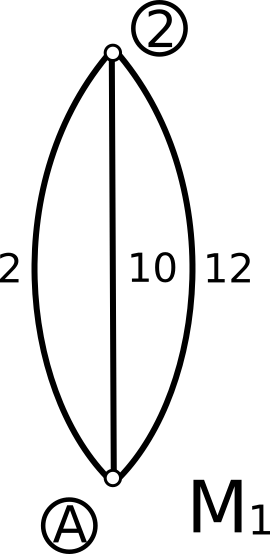
\includegraphics[width=0.16\textwidth]{images/ceyhun-167-fig01}&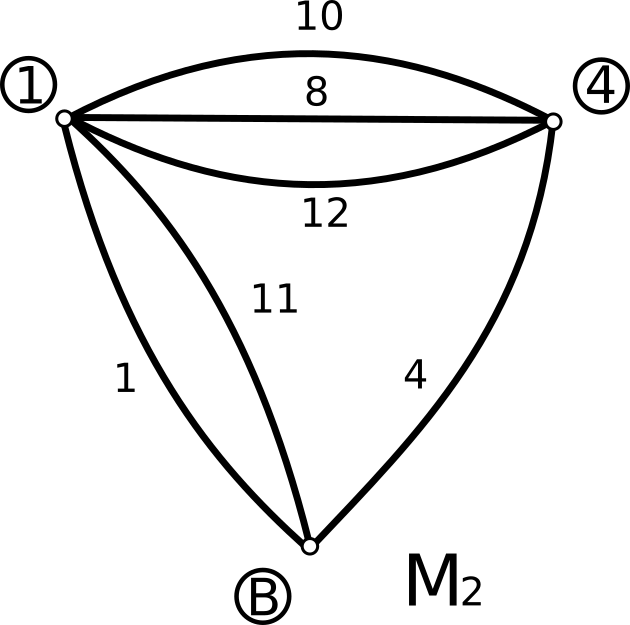
\includegraphics[width=0.36\textwidth]{images/ceyhun-167-fig02} &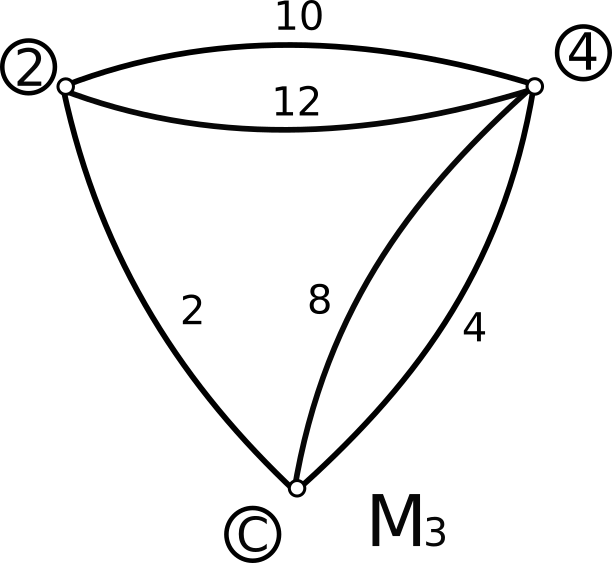
\includegraphics[width=0.36\textwidth]{images/ceyhun-167-fig03} \\
\end{tabular}
\\
\begin{tabular}{ l l l }
 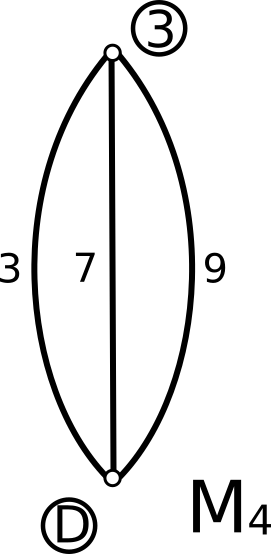
\includegraphics[width=0.16\textwidth]{images/ceyhun-167-fig04}&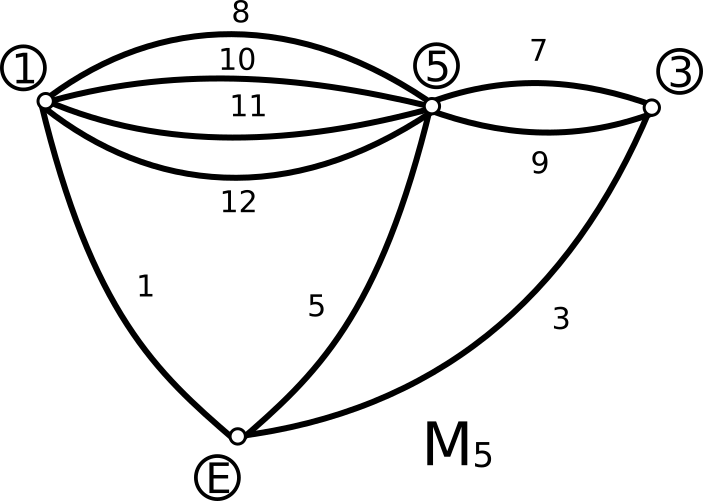
\includegraphics[width=0.54\textwidth]{images/ceyhun-167-fig05} &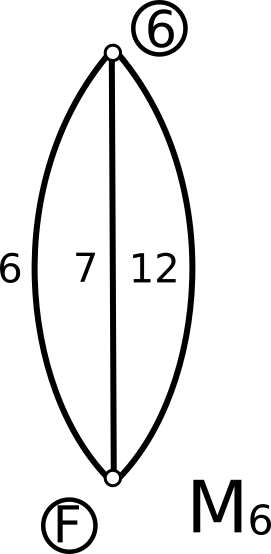
\includegraphics[width=0.16\textwidth]{images/ceyhun-167-fig06} \\
\end{tabular}
\\
(a) \quad\quad\quad\quad
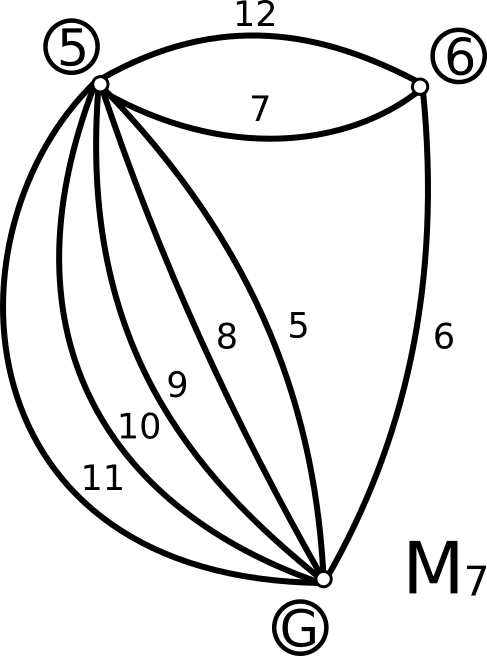
\includegraphics[width=0.3\textwidth]{images/ceyhun-167-fig07}
\end{document}